
% Default to the notebook output style

    


% Inherit from the specified cell style.




    
\documentclass[11pt]{article}

    
    
    \usepackage[T1]{fontenc}
    % Nicer default font (+ math font) than Computer Modern for most use cases
    \usepackage{mathpazo}

    % Basic figure setup, for now with no caption control since it's done
    % automatically by Pandoc (which extracts ![](path) syntax from Markdown).
    \usepackage{graphicx}
    % We will generate all images so they have a width \maxwidth. This means
    % that they will get their normal width if they fit onto the page, but
    % are scaled down if they would overflow the margins.
    \makeatletter
    \def\maxwidth{\ifdim\Gin@nat@width>\linewidth\linewidth
    \else\Gin@nat@width\fi}
    \makeatother
    \let\Oldincludegraphics\includegraphics
    % Set max figure width to be 80% of text width, for now hardcoded.
    \renewcommand{\includegraphics}[1]{\Oldincludegraphics[width=.8\maxwidth]{#1}}
    % Ensure that by default, figures have no caption (until we provide a
    % proper Figure object with a Caption API and a way to capture that
    % in the conversion process - todo).
    \usepackage{caption}
    \DeclareCaptionLabelFormat{nolabel}{}
    \captionsetup{labelformat=nolabel}

    \usepackage{adjustbox} % Used to constrain images to a maximum size 
    \usepackage{xcolor} % Allow colors to be defined
    \usepackage{enumerate} % Needed for markdown enumerations to work
    \usepackage{geometry} % Used to adjust the document margins
    \usepackage{amsmath} % Equations
    \usepackage{amssymb} % Equations
    \usepackage{textcomp} % defines textquotesingle
    % Hack from http://tex.stackexchange.com/a/47451/13684:
    \AtBeginDocument{%
        \def\PYZsq{\textquotesingle}% Upright quotes in Pygmentized code
    }
    \usepackage{upquote} % Upright quotes for verbatim code
    \usepackage{eurosym} % defines \euro
    \usepackage[mathletters]{ucs} % Extended unicode (utf-8) support
    \usepackage[utf8x]{inputenc} % Allow utf-8 characters in the tex document
    \usepackage{fancyvrb} % verbatim replacement that allows latex
    \usepackage{grffile} % extends the file name processing of package graphics 
                         % to support a larger range 
    % The hyperref package gives us a pdf with properly built
    % internal navigation ('pdf bookmarks' for the table of contents,
    % internal cross-reference links, web links for URLs, etc.)
    \usepackage{hyperref}
    \usepackage{longtable} % longtable support required by pandoc >1.10
    \usepackage{booktabs}  % table support for pandoc > 1.12.2
    \usepackage[inline]{enumitem} % IRkernel/repr support (it uses the enumerate* environment)
    \usepackage[normalem]{ulem} % ulem is needed to support strikethroughs (\sout)
                                % normalem makes italics be italics, not underlines
    

    
    
    % Colors for the hyperref package
    \definecolor{urlcolor}{rgb}{0,.145,.698}
    \definecolor{linkcolor}{rgb}{.71,0.21,0.01}
    \definecolor{citecolor}{rgb}{.12,.54,.11}

    % ANSI colors
    \definecolor{ansi-black}{HTML}{3E424D}
    \definecolor{ansi-black-intense}{HTML}{282C36}
    \definecolor{ansi-red}{HTML}{E75C58}
    \definecolor{ansi-red-intense}{HTML}{B22B31}
    \definecolor{ansi-green}{HTML}{00A250}
    \definecolor{ansi-green-intense}{HTML}{007427}
    \definecolor{ansi-yellow}{HTML}{DDB62B}
    \definecolor{ansi-yellow-intense}{HTML}{B27D12}
    \definecolor{ansi-blue}{HTML}{208FFB}
    \definecolor{ansi-blue-intense}{HTML}{0065CA}
    \definecolor{ansi-magenta}{HTML}{D160C4}
    \definecolor{ansi-magenta-intense}{HTML}{A03196}
    \definecolor{ansi-cyan}{HTML}{60C6C8}
    \definecolor{ansi-cyan-intense}{HTML}{258F8F}
    \definecolor{ansi-white}{HTML}{C5C1B4}
    \definecolor{ansi-white-intense}{HTML}{A1A6B2}

    % commands and environments needed by pandoc snippets
    % extracted from the output of `pandoc -s`
    \providecommand{\tightlist}{%
      \setlength{\itemsep}{0pt}\setlength{\parskip}{0pt}}
    \DefineVerbatimEnvironment{Highlighting}{Verbatim}{commandchars=\\\{\}}
    % Add ',fontsize=\small' for more characters per line
    \newenvironment{Shaded}{}{}
    \newcommand{\KeywordTok}[1]{\textcolor[rgb]{0.00,0.44,0.13}{\textbf{{#1}}}}
    \newcommand{\DataTypeTok}[1]{\textcolor[rgb]{0.56,0.13,0.00}{{#1}}}
    \newcommand{\DecValTok}[1]{\textcolor[rgb]{0.25,0.63,0.44}{{#1}}}
    \newcommand{\BaseNTok}[1]{\textcolor[rgb]{0.25,0.63,0.44}{{#1}}}
    \newcommand{\FloatTok}[1]{\textcolor[rgb]{0.25,0.63,0.44}{{#1}}}
    \newcommand{\CharTok}[1]{\textcolor[rgb]{0.25,0.44,0.63}{{#1}}}
    \newcommand{\StringTok}[1]{\textcolor[rgb]{0.25,0.44,0.63}{{#1}}}
    \newcommand{\CommentTok}[1]{\textcolor[rgb]{0.38,0.63,0.69}{\textit{{#1}}}}
    \newcommand{\OtherTok}[1]{\textcolor[rgb]{0.00,0.44,0.13}{{#1}}}
    \newcommand{\AlertTok}[1]{\textcolor[rgb]{1.00,0.00,0.00}{\textbf{{#1}}}}
    \newcommand{\FunctionTok}[1]{\textcolor[rgb]{0.02,0.16,0.49}{{#1}}}
    \newcommand{\RegionMarkerTok}[1]{{#1}}
    \newcommand{\ErrorTok}[1]{\textcolor[rgb]{1.00,0.00,0.00}{\textbf{{#1}}}}
    \newcommand{\NormalTok}[1]{{#1}}
    
    % Additional commands for more recent versions of Pandoc
    \newcommand{\ConstantTok}[1]{\textcolor[rgb]{0.53,0.00,0.00}{{#1}}}
    \newcommand{\SpecialCharTok}[1]{\textcolor[rgb]{0.25,0.44,0.63}{{#1}}}
    \newcommand{\VerbatimStringTok}[1]{\textcolor[rgb]{0.25,0.44,0.63}{{#1}}}
    \newcommand{\SpecialStringTok}[1]{\textcolor[rgb]{0.73,0.40,0.53}{{#1}}}
    \newcommand{\ImportTok}[1]{{#1}}
    \newcommand{\DocumentationTok}[1]{\textcolor[rgb]{0.73,0.13,0.13}{\textit{{#1}}}}
    \newcommand{\AnnotationTok}[1]{\textcolor[rgb]{0.38,0.63,0.69}{\textbf{\textit{{#1}}}}}
    \newcommand{\CommentVarTok}[1]{\textcolor[rgb]{0.38,0.63,0.69}{\textbf{\textit{{#1}}}}}
    \newcommand{\VariableTok}[1]{\textcolor[rgb]{0.10,0.09,0.49}{{#1}}}
    \newcommand{\ControlFlowTok}[1]{\textcolor[rgb]{0.00,0.44,0.13}{\textbf{{#1}}}}
    \newcommand{\OperatorTok}[1]{\textcolor[rgb]{0.40,0.40,0.40}{{#1}}}
    \newcommand{\BuiltInTok}[1]{{#1}}
    \newcommand{\ExtensionTok}[1]{{#1}}
    \newcommand{\PreprocessorTok}[1]{\textcolor[rgb]{0.74,0.48,0.00}{{#1}}}
    \newcommand{\AttributeTok}[1]{\textcolor[rgb]{0.49,0.56,0.16}{{#1}}}
    \newcommand{\InformationTok}[1]{\textcolor[rgb]{0.38,0.63,0.69}{\textbf{\textit{{#1}}}}}
    \newcommand{\WarningTok}[1]{\textcolor[rgb]{0.38,0.63,0.69}{\textbf{\textit{{#1}}}}}
    
    
    % Define a nice break command that doesn't care if a line doesn't already
    % exist.
    \def\br{\hspace*{\fill} \\* }
    % Math Jax compatability definitions
    \def\gt{>}
    \def\lt{<}
    % Document parameters
    \title{deep\_learning\_I}
    
    
    

    % Pygments definitions
    
\makeatletter
\def\PY@reset{\let\PY@it=\relax \let\PY@bf=\relax%
    \let\PY@ul=\relax \let\PY@tc=\relax%
    \let\PY@bc=\relax \let\PY@ff=\relax}
\def\PY@tok#1{\csname PY@tok@#1\endcsname}
\def\PY@toks#1+{\ifx\relax#1\empty\else%
    \PY@tok{#1}\expandafter\PY@toks\fi}
\def\PY@do#1{\PY@bc{\PY@tc{\PY@ul{%
    \PY@it{\PY@bf{\PY@ff{#1}}}}}}}
\def\PY#1#2{\PY@reset\PY@toks#1+\relax+\PY@do{#2}}

\expandafter\def\csname PY@tok@w\endcsname{\def\PY@tc##1{\textcolor[rgb]{0.73,0.73,0.73}{##1}}}
\expandafter\def\csname PY@tok@c\endcsname{\let\PY@it=\textit\def\PY@tc##1{\textcolor[rgb]{0.25,0.50,0.50}{##1}}}
\expandafter\def\csname PY@tok@cp\endcsname{\def\PY@tc##1{\textcolor[rgb]{0.74,0.48,0.00}{##1}}}
\expandafter\def\csname PY@tok@k\endcsname{\let\PY@bf=\textbf\def\PY@tc##1{\textcolor[rgb]{0.00,0.50,0.00}{##1}}}
\expandafter\def\csname PY@tok@kp\endcsname{\def\PY@tc##1{\textcolor[rgb]{0.00,0.50,0.00}{##1}}}
\expandafter\def\csname PY@tok@kt\endcsname{\def\PY@tc##1{\textcolor[rgb]{0.69,0.00,0.25}{##1}}}
\expandafter\def\csname PY@tok@o\endcsname{\def\PY@tc##1{\textcolor[rgb]{0.40,0.40,0.40}{##1}}}
\expandafter\def\csname PY@tok@ow\endcsname{\let\PY@bf=\textbf\def\PY@tc##1{\textcolor[rgb]{0.67,0.13,1.00}{##1}}}
\expandafter\def\csname PY@tok@nb\endcsname{\def\PY@tc##1{\textcolor[rgb]{0.00,0.50,0.00}{##1}}}
\expandafter\def\csname PY@tok@nf\endcsname{\def\PY@tc##1{\textcolor[rgb]{0.00,0.00,1.00}{##1}}}
\expandafter\def\csname PY@tok@nc\endcsname{\let\PY@bf=\textbf\def\PY@tc##1{\textcolor[rgb]{0.00,0.00,1.00}{##1}}}
\expandafter\def\csname PY@tok@nn\endcsname{\let\PY@bf=\textbf\def\PY@tc##1{\textcolor[rgb]{0.00,0.00,1.00}{##1}}}
\expandafter\def\csname PY@tok@ne\endcsname{\let\PY@bf=\textbf\def\PY@tc##1{\textcolor[rgb]{0.82,0.25,0.23}{##1}}}
\expandafter\def\csname PY@tok@nv\endcsname{\def\PY@tc##1{\textcolor[rgb]{0.10,0.09,0.49}{##1}}}
\expandafter\def\csname PY@tok@no\endcsname{\def\PY@tc##1{\textcolor[rgb]{0.53,0.00,0.00}{##1}}}
\expandafter\def\csname PY@tok@nl\endcsname{\def\PY@tc##1{\textcolor[rgb]{0.63,0.63,0.00}{##1}}}
\expandafter\def\csname PY@tok@ni\endcsname{\let\PY@bf=\textbf\def\PY@tc##1{\textcolor[rgb]{0.60,0.60,0.60}{##1}}}
\expandafter\def\csname PY@tok@na\endcsname{\def\PY@tc##1{\textcolor[rgb]{0.49,0.56,0.16}{##1}}}
\expandafter\def\csname PY@tok@nt\endcsname{\let\PY@bf=\textbf\def\PY@tc##1{\textcolor[rgb]{0.00,0.50,0.00}{##1}}}
\expandafter\def\csname PY@tok@nd\endcsname{\def\PY@tc##1{\textcolor[rgb]{0.67,0.13,1.00}{##1}}}
\expandafter\def\csname PY@tok@s\endcsname{\def\PY@tc##1{\textcolor[rgb]{0.73,0.13,0.13}{##1}}}
\expandafter\def\csname PY@tok@sd\endcsname{\let\PY@it=\textit\def\PY@tc##1{\textcolor[rgb]{0.73,0.13,0.13}{##1}}}
\expandafter\def\csname PY@tok@si\endcsname{\let\PY@bf=\textbf\def\PY@tc##1{\textcolor[rgb]{0.73,0.40,0.53}{##1}}}
\expandafter\def\csname PY@tok@se\endcsname{\let\PY@bf=\textbf\def\PY@tc##1{\textcolor[rgb]{0.73,0.40,0.13}{##1}}}
\expandafter\def\csname PY@tok@sr\endcsname{\def\PY@tc##1{\textcolor[rgb]{0.73,0.40,0.53}{##1}}}
\expandafter\def\csname PY@tok@ss\endcsname{\def\PY@tc##1{\textcolor[rgb]{0.10,0.09,0.49}{##1}}}
\expandafter\def\csname PY@tok@sx\endcsname{\def\PY@tc##1{\textcolor[rgb]{0.00,0.50,0.00}{##1}}}
\expandafter\def\csname PY@tok@m\endcsname{\def\PY@tc##1{\textcolor[rgb]{0.40,0.40,0.40}{##1}}}
\expandafter\def\csname PY@tok@gh\endcsname{\let\PY@bf=\textbf\def\PY@tc##1{\textcolor[rgb]{0.00,0.00,0.50}{##1}}}
\expandafter\def\csname PY@tok@gu\endcsname{\let\PY@bf=\textbf\def\PY@tc##1{\textcolor[rgb]{0.50,0.00,0.50}{##1}}}
\expandafter\def\csname PY@tok@gd\endcsname{\def\PY@tc##1{\textcolor[rgb]{0.63,0.00,0.00}{##1}}}
\expandafter\def\csname PY@tok@gi\endcsname{\def\PY@tc##1{\textcolor[rgb]{0.00,0.63,0.00}{##1}}}
\expandafter\def\csname PY@tok@gr\endcsname{\def\PY@tc##1{\textcolor[rgb]{1.00,0.00,0.00}{##1}}}
\expandafter\def\csname PY@tok@ge\endcsname{\let\PY@it=\textit}
\expandafter\def\csname PY@tok@gs\endcsname{\let\PY@bf=\textbf}
\expandafter\def\csname PY@tok@gp\endcsname{\let\PY@bf=\textbf\def\PY@tc##1{\textcolor[rgb]{0.00,0.00,0.50}{##1}}}
\expandafter\def\csname PY@tok@go\endcsname{\def\PY@tc##1{\textcolor[rgb]{0.53,0.53,0.53}{##1}}}
\expandafter\def\csname PY@tok@gt\endcsname{\def\PY@tc##1{\textcolor[rgb]{0.00,0.27,0.87}{##1}}}
\expandafter\def\csname PY@tok@err\endcsname{\def\PY@bc##1{\setlength{\fboxsep}{0pt}\fcolorbox[rgb]{1.00,0.00,0.00}{1,1,1}{\strut ##1}}}
\expandafter\def\csname PY@tok@kc\endcsname{\let\PY@bf=\textbf\def\PY@tc##1{\textcolor[rgb]{0.00,0.50,0.00}{##1}}}
\expandafter\def\csname PY@tok@kd\endcsname{\let\PY@bf=\textbf\def\PY@tc##1{\textcolor[rgb]{0.00,0.50,0.00}{##1}}}
\expandafter\def\csname PY@tok@kn\endcsname{\let\PY@bf=\textbf\def\PY@tc##1{\textcolor[rgb]{0.00,0.50,0.00}{##1}}}
\expandafter\def\csname PY@tok@kr\endcsname{\let\PY@bf=\textbf\def\PY@tc##1{\textcolor[rgb]{0.00,0.50,0.00}{##1}}}
\expandafter\def\csname PY@tok@bp\endcsname{\def\PY@tc##1{\textcolor[rgb]{0.00,0.50,0.00}{##1}}}
\expandafter\def\csname PY@tok@fm\endcsname{\def\PY@tc##1{\textcolor[rgb]{0.00,0.00,1.00}{##1}}}
\expandafter\def\csname PY@tok@vc\endcsname{\def\PY@tc##1{\textcolor[rgb]{0.10,0.09,0.49}{##1}}}
\expandafter\def\csname PY@tok@vg\endcsname{\def\PY@tc##1{\textcolor[rgb]{0.10,0.09,0.49}{##1}}}
\expandafter\def\csname PY@tok@vi\endcsname{\def\PY@tc##1{\textcolor[rgb]{0.10,0.09,0.49}{##1}}}
\expandafter\def\csname PY@tok@vm\endcsname{\def\PY@tc##1{\textcolor[rgb]{0.10,0.09,0.49}{##1}}}
\expandafter\def\csname PY@tok@sa\endcsname{\def\PY@tc##1{\textcolor[rgb]{0.73,0.13,0.13}{##1}}}
\expandafter\def\csname PY@tok@sb\endcsname{\def\PY@tc##1{\textcolor[rgb]{0.73,0.13,0.13}{##1}}}
\expandafter\def\csname PY@tok@sc\endcsname{\def\PY@tc##1{\textcolor[rgb]{0.73,0.13,0.13}{##1}}}
\expandafter\def\csname PY@tok@dl\endcsname{\def\PY@tc##1{\textcolor[rgb]{0.73,0.13,0.13}{##1}}}
\expandafter\def\csname PY@tok@s2\endcsname{\def\PY@tc##1{\textcolor[rgb]{0.73,0.13,0.13}{##1}}}
\expandafter\def\csname PY@tok@sh\endcsname{\def\PY@tc##1{\textcolor[rgb]{0.73,0.13,0.13}{##1}}}
\expandafter\def\csname PY@tok@s1\endcsname{\def\PY@tc##1{\textcolor[rgb]{0.73,0.13,0.13}{##1}}}
\expandafter\def\csname PY@tok@mb\endcsname{\def\PY@tc##1{\textcolor[rgb]{0.40,0.40,0.40}{##1}}}
\expandafter\def\csname PY@tok@mf\endcsname{\def\PY@tc##1{\textcolor[rgb]{0.40,0.40,0.40}{##1}}}
\expandafter\def\csname PY@tok@mh\endcsname{\def\PY@tc##1{\textcolor[rgb]{0.40,0.40,0.40}{##1}}}
\expandafter\def\csname PY@tok@mi\endcsname{\def\PY@tc##1{\textcolor[rgb]{0.40,0.40,0.40}{##1}}}
\expandafter\def\csname PY@tok@il\endcsname{\def\PY@tc##1{\textcolor[rgb]{0.40,0.40,0.40}{##1}}}
\expandafter\def\csname PY@tok@mo\endcsname{\def\PY@tc##1{\textcolor[rgb]{0.40,0.40,0.40}{##1}}}
\expandafter\def\csname PY@tok@ch\endcsname{\let\PY@it=\textit\def\PY@tc##1{\textcolor[rgb]{0.25,0.50,0.50}{##1}}}
\expandafter\def\csname PY@tok@cm\endcsname{\let\PY@it=\textit\def\PY@tc##1{\textcolor[rgb]{0.25,0.50,0.50}{##1}}}
\expandafter\def\csname PY@tok@cpf\endcsname{\let\PY@it=\textit\def\PY@tc##1{\textcolor[rgb]{0.25,0.50,0.50}{##1}}}
\expandafter\def\csname PY@tok@c1\endcsname{\let\PY@it=\textit\def\PY@tc##1{\textcolor[rgb]{0.25,0.50,0.50}{##1}}}
\expandafter\def\csname PY@tok@cs\endcsname{\let\PY@it=\textit\def\PY@tc##1{\textcolor[rgb]{0.25,0.50,0.50}{##1}}}

\def\PYZbs{\char`\\}
\def\PYZus{\char`\_}
\def\PYZob{\char`\{}
\def\PYZcb{\char`\}}
\def\PYZca{\char`\^}
\def\PYZam{\char`\&}
\def\PYZlt{\char`\<}
\def\PYZgt{\char`\>}
\def\PYZsh{\char`\#}
\def\PYZpc{\char`\%}
\def\PYZdl{\char`\$}
\def\PYZhy{\char`\-}
\def\PYZsq{\char`\'}
\def\PYZdq{\char`\"}
\def\PYZti{\char`\~}
% for compatibility with earlier versions
\def\PYZat{@}
\def\PYZlb{[}
\def\PYZrb{]}
\makeatother


    % Exact colors from NB
    \definecolor{incolor}{rgb}{0.0, 0.0, 0.5}
    \definecolor{outcolor}{rgb}{0.545, 0.0, 0.0}



    
    % Prevent overflowing lines due to hard-to-break entities
    \sloppy 
    % Setup hyperref package
    \hypersetup{
      breaklinks=true,  % so long urls are correctly broken across lines
      colorlinks=true,
      urlcolor=urlcolor,
      linkcolor=linkcolor,
      citecolor=citecolor,
      }
    % Slightly bigger margins than the latex defaults
    
    \geometry{verbose,tmargin=1in,bmargin=1in,lmargin=1in,rmargin=1in}
    
    

    \begin{document}
    
    
    \maketitle
    
    

    
    \#

Deep Learning and Text Analytics

References: - General introduction -
http://ufldl.stanford.edu/tutorial/supervised/MultiLayerNeuralNetworks/
- Word vector: - https://code.google.com/archive/p/word2vec/ - Keras
tutorial -
https://machinelearningmastery.com/tutorial-first-neural-network-python-keras/
- CNN -
http://www.wildml.com/2015/11/understanding-convolutional-neural-networks-for-nlp/

    \hypertarget{agenda}{%
\subsection{1. Agenda}\label{agenda}}

\begin{itemize}
\tightlist
\item
  Introduction to neural networks
\item
  Word/Document Vectors (vector representation of
  words/phrases/paragraphs)
\item
  Convolutionary neural network (CNN)
\item
  Application of CNN in text classification
\end{itemize}

    \hypertarget{introduction-neural-networks}{%
\subsection{2. Introduction neural
networks}\label{introduction-neural-networks}}

\begin{itemize}
\tightlist
\item
  A neural network is a computational model inspired by the way
  biological neural networks in the human brain process information.
\item
  Neural networks have been widely applied in speech recognition,
  computer vision and text processing
\end{itemize}

    \hypertarget{single-neuron}{%
\subsubsection{2.1. Single Neuron}\label{single-neuron}}

 \[h_{W,b}(x)=f(w_1x_1+w_2x_2+w_3x_3+b)\] - Basic components: -
\textbf{input} (\(X\)): \([x_1, x_2, x_3]\) - \textbf{weight} (\(W\)):
\([w_1, w_2, w_3]\) - \textbf{bias}: \(b\) - \textbf{activation}
function: \(f\) - Different activation functions: - \textbf{Sigmoid}
(logistic function): takes a real-valued input and squashes it to range
{[}0,1{]}. \[f(z)=\frac{1}{1+e^{-z}}\], where
\(z=w_1x_1+w_2x_2+w_3x_3+b\) - Tanh (hyperbolic tangent): takes a
real-valued input and squashes it to the range {[}-1, 1{]}.
\[f(z)=tanh(z)=\frac{e^z-e^{-z}}{e^z+e^{-z}}\] - ReLU (Rectified Linear
Unit): \[f(z)=max(0,z)\]\\
- \textbf{Softmax} (normalized exponential function): a generalization
of the logistic function. If \(z=[z_1, z_2, ..., z_k]\) is a
\(k\)-dimensional vector,
\[f(z)_{j \in k}=\frac{e^{z_j}}{\sum_{i=1}^k{e^{z_i}}}\] -
\(f(z)_{j} \in [0,1]\) - \$\sum\emph{\{j \in k\} \{f(z)}\{j\}\} =1 \$ -
\(f(z)_{j}\) is treated as the \textbf{probability} of component \(j\),
a probability distribution over \(k\) different possible outcomes -
e.g.~in multi-label classification, softmax gives a probability of each
label

    \hypertarget{neural-network-model}{%
\subsubsection{2.2 Neural Network Model}\label{neural-network-model}}

\begin{itemize}
\tightlist
\item
  A neural network is composed of many simple neurons, so that the
  output of a neuron can be the input of another
\item
  The sample neural network model has 3 input nodes, 3 hidden units, and
  1 output unit

  \begin{itemize}
  \tightlist
  \item
    input layer: the leftmost layer
  \item
    outout layer: the rightmost layer (produce target, i.e.~prediction,
    classification)
  \item
    bias units: indicated by ``+1'' node
  \item
    hidden layer: the middle layer of nodes 
  \end{itemize}
\item
  \(W\), \(x\), and \(b\) usually represented as arrays
  (i.e.~vectorized)

  \begin{itemize}
  \tightlist
  \item
    \(w_{ij}^{(l)}\): the weight associated with the link from unit
    \(j\) in layer \(l\) to unit \(i\) in layer \(l+1\)
  \item
    \(W^{(1)} \in \mathbb{R}^{3\text{x}3}\),
    \(W^{(2)} \in \mathbb{R}^{1\text{x}3}\),
    \(b^{(1)} \in \mathbb{R}^{3\text{x}1}\),
    \(b^{(2)} \in \mathbb{R}^{1\text{x}1}\)
  \item
    Note \(W^{(l)}x\) is the dot product between \(W^{(l)}\) and \(x\),
    i.e. \(W^{(l)} \cdot x\)
  \end{itemize}
\item
  If a neural network contains more than 1 hidden layer, it's called a
  \textbf{deep neural network} (\textbf{deep learning})
\item
  Training a neural network model is to find \(W\) and \(b\) that
  optimize some \textbf{cost function}, given tranining samples (X,Y),
  where X and Y can be multi-dimensional
\end{itemize}

    \hypertarget{cost-function}{%
\subsubsection{2.3. Cost function}\label{cost-function}}

\begin{itemize}
\tightlist
\item
  Training set: m samples denoted as
  \((X,Y)={(x^{(1)}, y^{(1)}), (x^{(2)}, y^{(2)}), ..., (x^{(m)}, y^{(m)})}\)
\item
  A typical cost function: \textbf{mean\_squared\_error}

  \begin{itemize}
  \tightlist
  \item
    Sum of square error: \(J(W,b;x,y)=\frac{1}{2}||h_{W,b}(x)-y||^2\)
  \item
    Regularization (square of each weight, or L2):
    \(\sum_{i, j, l}(w_{ij}^{(l)})^2\). An important mechanism to
    prevent overfitting
  \item
    Cost function:
    \[J(W,b)=\frac{1}{m}\sum_i^m{(\frac{1}{2}||h_{W,b}(x)-y||^2)}+ \frac{\lambda}{2}\sum_{i, j, l}(w_{ij}^{(l)})^2\],
    where \(\lambda\) is \textbf{regularization coefficient}
  \end{itemize}
\item
  Other popular cost functions

  \begin{itemize}
  \tightlist
  \item
    \textbf{Cross-entropy cost}

    \begin{itemize}
    \tightlist
    \item
      Let's assume a single neuron with sigmoid activation function 
    \item
      Let \(\widehat y=h_{W,b}(x)\), the prediction of true value \(y\).
      \(\widehat y, y \in [0,1]\).
    \item
      Then cross-entrophy cost is defined as:
      \[J=-\frac{1}{m}\sum_{i=1}^m{y_i\ln{\widehat y_i}+(1-y_i)\ln{(1-\widehat y_i)}}\]
    \item
      What makes cross-entropy a good cost function

      \begin{itemize}
      \tightlist
      \item
        It's non-negative
      \item
        if the neuron's output \(\widehat y\) is close to the actual
        value \(y\) (0 or 1) for all training inputs, then the
        cross-entropy will be close to zero
      \end{itemize}
    \end{itemize}
  \end{itemize}
\item
  For comparison between ``Sum of Square error'' and ``Cross-entropy
  cost'', read http://neuralnetworksanddeeplearning.com/chap3.html
\end{itemize}

    \hypertarget{gradient-descent}{%
\subsubsection{2.4. Gradient Descent}\label{gradient-descent}}

\begin{itemize}
\tightlist
\item
  An optimization algorithm used to find the values of parameters
  (\(W, b\)) of a function (\(J\)) that minimizes a cost function
  (\(J(W,b)\).
\item
  It is best used when the parameters cannot be calculated analytically
  (e.g.~using linear algebra) and must be searched for by an
  optimization algorithm resource:
  https://www.analyticsvidhya.com/blog/2017/03/introduction-to-gradient-descent-algorithm-along-its-variants/
\item
  It uses derivatives of cost function to determine the direction to
  move the parameter values in order to get a lower cost on the next
  iteration
\item
  Procedure:

  \begin{enumerate}
  \def\labelenumi{\arabic{enumi}.}
  \tightlist
  \item
    initialize \(W\) with random values
  \item
    given samples (X,Y) as inputs, calculate dirivatives of cost
    function with regard to every parameter \(w_{ij}^{(l)}\), i.e.
    \(\frac{\partial{J}}{\partial{w_{ij}^{(l)}}}\)
  \item
    update parameters by
    \((w_{ij}^{(l)})^{'}=w_{ij}^{(l)}-\alpha*\frac{\partial{J}}{\partial{w_{ij}^{(l)}}}\),
    where \(\alpha\) is the learning rate
  \item
    repeat steps 2-3 until \(w_{ij}^{(l)}\) converges
  \end{enumerate}
\item
  \textbf{Learning rate \(\alpha\)}

  \begin{itemize}
  \tightlist
  \item
    It's critical to pick the right learning rate. Big \(\alpha\) or
    small \(\alpha\)?
  \item
    \(\alpha\) may need to be adapted as learning unfolds
  \end{itemize}
\item
  Challenges of Gradient Descent

  \begin{itemize}
  \tightlist
  \item
    It is expensive to compute
    \(\frac{1}{m}\sum_i^m{(\frac{1}{2}||h_{W,b}(x_i)-y_i||^2)}\) for all
    samples in each round
  \item
    It is difficult to compute
    \(\frac{\partial{J}}{\partial{w_{ij}^{(l)}}}\) if a neural netowrk
    has many layers
  \end{itemize}
\end{itemize}

    \hypertarget{stochastic-gradient-descent}{%
\subsubsection{2.5. Stochastic Gradient
Descent}\label{stochastic-gradient-descent}}

\begin{itemize}
\tightlist
\item
  Estimate of cost function using a subset of randomly chosen training
  samples (mini-batch) instead of the entire training set
\item
  Procedure:

  \begin{enumerate}
  \def\labelenumi{\arabic{enumi}.}
  \tightlist
  \item
    pick a randomly selected mini-batch, train with them and update
    \(W, b\),
  \item
    repeat step (1) with another randomly selected mini-batch until the
    training set is exhausted (i.e.~complete an epoch),
  \item
    start over with another epoch until \(W, b\) converge
  \end{enumerate}
\item
  \textbf{Hyperparameters} (parameters that control the learning of
  \(W, b\))

  \begin{itemize}
  \tightlist
  \item
    \textbf{Batch size}: the size of samples selected for each iteration
  \item
    \textbf{Epoches}: One epoch means one complete pass through the
    whole training set. Ususally we need to use many epoches until
    \(W, b\) converge
  \item
    e.g.~if your sample size is 1000, and your batch size is 200, how
    many iterations are needed for one epoch?
  \item
    e.g.~if you set \# of epoches to 5, how many times in total you
    update \(W, b\)?
  \end{itemize}
\end{itemize}

    \hypertarget{backpropagation-algorithm-the-efficient-way-to-calcluate-gradients-i.e.partial-derivatives}{%
\paragraph{2.6. Backpropagation Algorithm -- The efficient way to
calcluate gradients (i.e.~partial
derivatives)}\label{backpropagation-algorithm-the-efficient-way-to-calcluate-gradients-i.e.partial-derivatives}}

\begin{longtable}[]{@{}cc@{}}
\toprule
\begin{minipage}[b]{0.47\columnwidth}\centering
Forward Propagation\strut
\end{minipage} & \begin{minipage}[b]{0.47\columnwidth}\centering
Backprogation\strut
\end{minipage}\tabularnewline
\midrule
\endhead
\begin{minipage}[t]{0.47\columnwidth}\centering
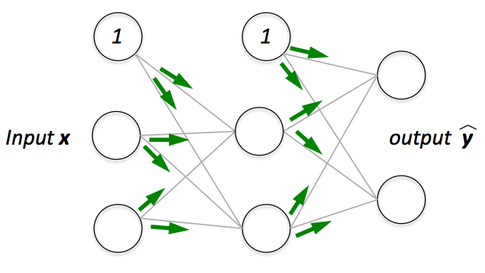
\includegraphics{forward-propagation.png}\strut
\end{minipage} & \begin{minipage}[t]{0.47\columnwidth}\centering
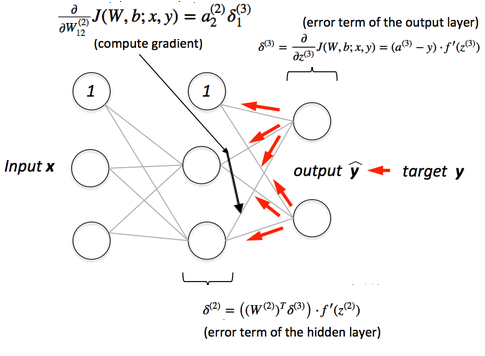
\includegraphics{backpropagation.png}\strut
\end{minipage}\tabularnewline
\begin{minipage}[t]{0.47\columnwidth}\centering
input signals are passing through each layer by multiplying the
weights\strut
\end{minipage} & \begin{minipage}[t]{0.47\columnwidth}\centering
backpropagate the error back to each layer proportional to perspective
weights, and update the weights based on attributed errors in hope to
correct the error\strut
\end{minipage}\tabularnewline
\bottomrule
\end{longtable}

\begin{itemize}
\tightlist
\item
  Algorithm:

  \begin{enumerate}
  \def\labelenumi{\arabic{enumi}.}
  \tightlist
  \item
    perform a feedforward pass, computing the activations for layers L2,
    L3, \ldots{} and so on up to the output layer
  \item
    for output layer \(n\),
    \(\delta^{(n)} = \frac{\partial}{\partial z^{(n)}}  J(W,b; x, y) = \frac{\partial}{\partial z^{(n)}}  \frac{1}{2} \left\|y - h_{W,b}(x)\right\|^2 = - (y - a^{(n)}) \cdot f'(z^{(n)})\)
  \item
    for \(l=n-1, n-2, ..., n-3, ..., 2\), \$ \delta\^{}\{(l)\} =
    \left((W\textsuperscript{\{(l)\})}T \delta\^{}\{(l+1)\}\right)
    \cdot f'(z\^{}\{(l)\})\$
  \item
    Compute the desired partial derivatives, which are given as: \$
    \frac{\partial}{\partial W_{ij}^{(l)}} J(W,b; x, y) =
    a\^{}\{(l)\}\_j \delta\_i\^{}\{(l+1)\}\$
    \(\frac{\partial}{\partial b_{i}^{(l)}} J(W,b; x, y) = \delta_i^{(l+1)}\)
  \end{enumerate}
\item
  Example:

  \begin{itemize}
  \item
    \(\delta^{(3)} = \frac{\partial}{\partial z^{(3)}} J(W,b; x, y) = (a^{(3)} - y) \cdot f'(z^{(3)})\)
  \item
    \$ \delta\^{}\{(2)\} = \left((W\textsuperscript{\{(2)\})}T
    \delta\^{}\{(3)\}\right) \cdot f'(z\^{}\{(2)\})\$
  \item
    \$ \frac{\partial}{\partial W_{12}^{(2)}} J(W,b; x, y) =
    a\^{}\{(2)\}\_2 \delta\_1\^{}\{(3)\}\$
  \end{itemize}
\end{itemize}

    \hypertarget{hyperparameters}{%
\subsubsection{2.7 Hyperparameters}\label{hyperparameters}}

\begin{itemize}
\tightlist
\item
  Hyperparameters are parameters that control the learning of \(w, b\)
  (our learning target)
\item
  Summary of hyperparameters:

  \begin{itemize}
  \tightlist
  \item
    Network structure:

    \begin{itemize}
    \tightlist
    \item
      number of hidden layers
    \item
      number of neurons of each layer
    \item
      activation fucntion of each layer
    \end{itemize}
  \item
    Learning rate (\(\alpha\))
  \item
    regularization coeffiecient (\(\lambda\))
  \item
    mini-batch size
  \item
    epoches
  \end{itemize}
\item
  For detailed explanation, watch:
  https://www.coursera.org/learn/neural-networks-deep-learning/lecture/TBvb5/parameters-vs-hyperparameters
\end{itemize}

    \hypertarget{develop-your-first-neural-network-model-with-keras}{%
\subsection{3. Develop your First Neural Network Model with
Keras}\label{develop-your-first-neural-network-model-with-keras}}

\begin{itemize}
\tightlist
\item
  Keras:

  \begin{itemize}
  \tightlist
  \item
    high-level library for neural network models
  \item
    It wraps the efficient numerical computation libraries Theano and
    TensorFlow
  \end{itemize}
\item
  Why Keras:

  \begin{itemize}
  \tightlist
  \item
    Simple to get started and keep going
  \item
    Written in python and higly modular; easy to expand
  \item
    Built-in modules for some sophisticated neural network models
  \end{itemize}
\item
  Installation

  \begin{itemize}
  \tightlist
  \item
    pip install keras (or pip install keras --upgrade if you already
    have it) to install the latest version
  \item
    pip install theano
  \item
    pip install tensorflow
  \item
    pip install np-utils
  \end{itemize}
\item
  Basic procedure

  \begin{enumerate}
  \def\labelenumi{\arabic{enumi}.}
  \tightlist
  \item
    Load data
  \item
    Define model
  \item
    Compile model
  \item
    Fit model
  \item
    Evaluate model
  \end{enumerate}
\end{itemize}

    \hypertarget{basic-keras-modeling-constructs}{%
\subsubsection{3.1. Basic Keras Modeling
Constructs}\label{basic-keras-modeling-constructs}}

\begin{itemize}
\tightlist
\item
  Sequential model: linear stack of layers
\item
  Layers

  \begin{itemize}
  \tightlist
  \item
    Dense: in a dense layer, each neuron is connected to neurons in the
    next layer
  \item
    Embedding
  \item
    Convolution
  \item
    MaxPooling
  \item
    \ldots{}
  \end{itemize}
\item
  Cost (loss) functions

  \begin{itemize}
  \tightlist
  \item
    mean\_squared\_error
  \item
    binary\_crossentropy
  \item
    categorical\_crossentropy
  \item
    \ldots{}
  \end{itemize}
\item
  Optimizer (i.e.~optimization algorithm)

  \begin{itemize}
  \tightlist
  \item
    SGD (Stochastic Gradient Descent): fixed learning rate in all
    iterations
  \item
    Adagrad: adapts the learning rate to the parameters, performing
    larger updates for infrequent, and smaller updates for frequent
    parameters
  \item
    Adam (Adaptive Moment Estimation): computes adaptive learning rates
    for each parameter.
  \end{itemize}
\item
  Metrics

  \begin{itemize}
  \tightlist
  \item
    accuracy: a ratio of correctly predicted samples to the total
    samples
  \item
    precision/recall/f1 through sklearn package
  \item
    Example:

    \begin{itemize}
    \tightlist
    \item
      acc: (90+85)/200=87\%
    \item
      prec:
    \item
      recall:
    \end{itemize}
  \end{itemize}
\end{itemize}

\begin{longtable}[]{@{}lrr@{}}
\toprule
& Predicted T & Predicted F\tabularnewline
\midrule
\endhead
Actual T & 90 & 10\tabularnewline
Actual F & 15 & 85\tabularnewline
\bottomrule
\end{longtable}

    \hypertarget{example}{%
\subsubsection{3.2. Example}\label{example}}

\begin{itemize}
\tightlist
\item
  Example: build a simple neural network model to predict diabetes using
  ``Pima Indians onset of diabetes database'' at
  http://archive.ics.uci.edu/ml/datasets/Pima+Indians+Diabetes

  \begin{itemize}
  \tightlist
  \item
    Columns 1-8: variables
  \item
    Column 9: class variable, 0 or 1
  \end{itemize}
\item
  A sequential model with 4 layers

  \begin{itemize}
  \tightlist
  \item
    each node is a tensor, a function of multidimensional arrays

    \begin{itemize}
    \tightlist
    \item
      Input (L1)
    \item
      L2 (hidden layer, dense)
    \item
      L3 (hidden layer, dense)
    \item
      Output (dense)
    \end{itemize}
  \item
    the model is a tensor graph (computation graph)
  \end{itemize}

  Training a deep learning model is a very empirical process. You may
  need to tune the hyperparameters in many iterations
\end{itemize}

    \begin{Verbatim}[commandchars=\\\{\}]
{\color{incolor}In [{\color{incolor}1}]:} \PY{c+c1}{\PYZsh{} set up interactive shell}
        \PY{k+kn}{from} \PY{n+nn}{IPython}\PY{n+nn}{.}\PY{n+nn}{core}\PY{n+nn}{.}\PY{n+nn}{interactiveshell} \PY{k}{import} \PY{n}{InteractiveShell}
        \PY{n}{InteractiveShell}\PY{o}{.}\PY{n}{ast\PYZus{}node\PYZus{}interactivity} \PY{o}{=} \PY{l+s+s2}{\PYZdq{}}\PY{l+s+s2}{all}\PY{l+s+s2}{\PYZdq{}}
\end{Verbatim}


    \begin{Verbatim}[commandchars=\\\{\}]
{\color{incolor}In [{\color{incolor}2}]:} \PY{c+c1}{\PYZsh{} Exercise 3.1. Load data}
        \PY{k+kn}{import} \PY{n+nn}{numpy} \PY{k}{as} \PY{n+nn}{np}
        \PY{k+kn}{import} \PY{n+nn}{pandas} \PY{k}{as} \PY{n+nn}{pd}
        
        \PY{c+c1}{\PYZsh{} Load data}
        \PY{n}{data}\PY{o}{=}\PY{n}{pd}\PY{o}{.}\PY{n}{read\PYZus{}csv}\PY{p}{(}\PY{l+s+s2}{\PYZdq{}}\PY{l+s+s2}{pima\PYZhy{}indians\PYZhy{}diabetes.csv}\PY{l+s+s2}{\PYZdq{}}\PY{p}{,}\PY{n}{header}\PY{o}{=}\PY{k+kc}{None}\PY{p}{)}
        \PY{n}{data}\PY{o}{.}\PY{n}{head}\PY{p}{(}\PY{p}{)}
        
        \PY{n}{data}\PY{p}{[}\PY{l+m+mi}{8}\PY{p}{]}\PY{o}{.}\PY{n}{value\PYZus{}counts}\PY{p}{(}\PY{p}{)}
        
        \PY{n}{X}\PY{o}{=}\PY{n}{data}\PY{o}{.}\PY{n}{values}\PY{p}{[}\PY{p}{:}\PY{p}{,}\PY{l+m+mi}{0}\PY{p}{:}\PY{l+m+mi}{8}\PY{p}{]}
        \PY{n}{y}\PY{o}{=}\PY{n}{data}\PY{o}{.}\PY{n}{values}\PY{p}{[}\PY{p}{:}\PY{p}{,}\PY{l+m+mi}{8}\PY{p}{]}
        \PY{n}{X}\PY{o}{.}\PY{n}{shape}
\end{Verbatim}


\begin{Verbatim}[commandchars=\\\{\}]
{\color{outcolor}Out[{\color{outcolor}2}]:}    0    1   2   3    4     5      6   7  8
        0  6  148  72  35    0  33.6  0.627  50  1
        1  1   85  66  29    0  26.6  0.351  31  0
        2  8  183  64   0    0  23.3  0.672  32  1
        3  1   89  66  23   94  28.1  0.167  21  0
        4  0  137  40  35  168  43.1  2.288  33  1
\end{Verbatim}
            
\begin{Verbatim}[commandchars=\\\{\}]
{\color{outcolor}Out[{\color{outcolor}2}]:} 0    500
        1    268
        Name: 8, dtype: int64
\end{Verbatim}
            
\begin{Verbatim}[commandchars=\\\{\}]
{\color{outcolor}Out[{\color{outcolor}2}]:} (768, 8)
\end{Verbatim}
            
    \begin{Verbatim}[commandchars=\\\{\}]
{\color{incolor}In [{\color{incolor}3}]:} \PY{c+c1}{\PYZsh{} Exercise 3.2. Create Model}
        
        \PY{c+c1}{\PYZsh{} sequential model is a linear stack of layers}
        \PY{k+kn}{from} \PY{n+nn}{keras}\PY{n+nn}{.}\PY{n+nn}{models} \PY{k}{import} \PY{n}{Sequential}
        
        \PY{c+c1}{\PYZsh{} in a dense layer which each neuron is connected to }
        \PY{c+c1}{\PYZsh{} each neuron in the next layer}
        \PY{k+kn}{from} \PY{n+nn}{keras}\PY{n+nn}{.}\PY{n+nn}{layers} \PY{k}{import} \PY{n}{Dense}
        
        \PY{c+c1}{\PYZsh{} import packages for L2 regularization}
        \PY{k+kn}{from} \PY{n+nn}{keras}\PY{n+nn}{.}\PY{n+nn}{regularizers} \PY{k}{import} \PY{n}{l2}
        
        \PY{c+c1}{\PYZsh{} fix random seed for reproducibility}
        \PY{n}{np}\PY{o}{.}\PY{n}{random}\PY{o}{.}\PY{n}{seed}\PY{p}{(}\PY{l+m+mi}{7}\PY{p}{)}
        
        \PY{c+c1}{\PYZsh{} set lambda (regularization coefficient)}
        \PY{n}{lam}\PY{o}{=}\PY{l+m+mf}{0.01}
        
        \PY{c+c1}{\PYZsh{} create a sequential model}
        \PY{n}{model} \PY{o}{=} \PY{n}{Sequential}\PY{p}{(}\PY{p}{)}
        
        \PY{c+c1}{\PYZsh{} add a dense layer with 12 neurons, 8 input variables}
        \PY{c+c1}{\PYZsh{} and rectifier activation function (relu)}
        \PY{c+c1}{\PYZsh{} and L2 regularization}
        \PY{c+c1}{\PYZsh{} how many parameters in this layer?}
        \PY{n}{model}\PY{o}{.}\PY{n}{add}\PY{p}{(}\PY{n}{Dense}\PY{p}{(}\PY{l+m+mi}{12}\PY{p}{,} \PY{n}{input\PYZus{}dim}\PY{o}{=}\PY{l+m+mi}{8}\PY{p}{,} \PY{n}{activation}\PY{o}{=}\PY{l+s+s1}{\PYZsq{}}\PY{l+s+s1}{relu}\PY{l+s+s1}{\PYZsq{}}\PY{p}{,} \PYZbs{}
                        \PY{n}{kernel\PYZus{}regularizer}\PY{o}{=}\PY{n}{l2}\PY{p}{(}\PY{n}{lam}\PY{p}{)}\PY{p}{,} \PY{n}{name}\PY{o}{=}\PY{l+s+s1}{\PYZsq{}}\PY{l+s+s1}{L2}\PY{l+s+s1}{\PYZsq{}}\PY{p}{)} \PY{p}{)}
        
        \PY{c+c1}{\PYZsh{} add another hidden layer with 8 neurons}
        \PY{n}{model}\PY{o}{.}\PY{n}{add}\PY{p}{(}\PY{n}{Dense}\PY{p}{(}\PY{l+m+mi}{8}\PY{p}{,} \PY{n}{activation}\PY{o}{=}\PY{l+s+s1}{\PYZsq{}}\PY{l+s+s1}{relu}\PY{l+s+s1}{\PYZsq{}}\PY{p}{,} \PYZbs{}
                        \PY{n}{kernel\PYZus{}regularizer}\PY{o}{=}\PY{n}{l2}\PY{p}{(}\PY{n}{lam}\PY{p}{)}\PY{p}{,}\PY{n}{name}\PY{o}{=}\PY{l+s+s1}{\PYZsq{}}\PY{l+s+s1}{L3}\PY{l+s+s1}{\PYZsq{}}\PY{p}{)} \PY{p}{)}
        
        \PY{c+c1}{\PYZsh{} add the output layer with sigmoid activation function}
        \PY{c+c1}{\PYZsh{} to return probability}
        \PY{n}{model}\PY{o}{.}\PY{n}{add}\PY{p}{(}\PY{n}{Dense}\PY{p}{(}\PY{l+m+mi}{1}\PY{p}{,} \PY{n}{activation}\PY{o}{=}\PY{l+s+s1}{\PYZsq{}}\PY{l+s+s1}{sigmoid}\PY{l+s+s1}{\PYZsq{}}\PY{p}{,} \PY{n}{name}\PY{o}{=}\PY{l+s+s1}{\PYZsq{}}\PY{l+s+s1}{Output}\PY{l+s+s1}{\PYZsq{}}\PY{p}{)}\PY{p}{)}
        
        \PY{c+c1}{\PYZsh{} compile the model using binary corss entropy cost function}
        \PY{c+c1}{\PYZsh{} adam optimizer and accuracy}
        \PY{n}{model}\PY{o}{.}\PY{n}{compile}\PY{p}{(}\PY{n}{loss}\PY{o}{=}\PY{l+s+s1}{\PYZsq{}}\PY{l+s+s1}{binary\PYZus{}crossentropy}\PY{l+s+s1}{\PYZsq{}}\PY{p}{,} \PYZbs{}
                      \PY{n}{optimizer}\PY{o}{=}\PY{l+s+s1}{\PYZsq{}}\PY{l+s+s1}{adam}\PY{l+s+s1}{\PYZsq{}}\PY{p}{,} \PY{n}{metrics}\PY{o}{=}\PY{p}{[}\PY{l+s+s1}{\PYZsq{}}\PY{l+s+s1}{accuracy}\PY{l+s+s1}{\PYZsq{}}\PY{p}{]}\PY{p}{)}
\end{Verbatim}


    \begin{Verbatim}[commandchars=\\\{\}]
Using TensorFlow backend.

    \end{Verbatim}

    \begin{Verbatim}[commandchars=\\\{\}]
{\color{incolor}In [{\color{incolor}4}]:} \PY{c+c1}{\PYZsh{} Exercise 3.3. Check model configuration}
        
        \PY{n}{model}\PY{o}{.}\PY{n}{summary}\PY{p}{(}\PY{p}{)}
        
        \PY{c+c1}{\PYZsh{} Show the model in a computation graph}
        \PY{c+c1}{\PYZsh{} it needs pydot and graphviz}
        \PY{c+c1}{\PYZsh{} don\PYZsq{}t worry if you don\PYZsq{}t have them installed}
        
        \PY{c+c1}{\PYZsh{}from keras.utils import plot\PYZus{}model}
        \PY{c+c1}{\PYZsh{}plot\PYZus{}model(model, to\PYZus{}file=\PYZsq{}model.png\PYZsq{})}
\end{Verbatim}


    \begin{Verbatim}[commandchars=\\\{\}]
\_\_\_\_\_\_\_\_\_\_\_\_\_\_\_\_\_\_\_\_\_\_\_\_\_\_\_\_\_\_\_\_\_\_\_\_\_\_\_\_\_\_\_\_\_\_\_\_\_\_\_\_\_\_\_\_\_\_\_\_\_\_\_\_\_
Layer (type)                 Output Shape              Param \#   
=================================================================
L2 (Dense)                   (None, 12)                108       
\_\_\_\_\_\_\_\_\_\_\_\_\_\_\_\_\_\_\_\_\_\_\_\_\_\_\_\_\_\_\_\_\_\_\_\_\_\_\_\_\_\_\_\_\_\_\_\_\_\_\_\_\_\_\_\_\_\_\_\_\_\_\_\_\_
L3 (Dense)                   (None, 8)                 104       
\_\_\_\_\_\_\_\_\_\_\_\_\_\_\_\_\_\_\_\_\_\_\_\_\_\_\_\_\_\_\_\_\_\_\_\_\_\_\_\_\_\_\_\_\_\_\_\_\_\_\_\_\_\_\_\_\_\_\_\_\_\_\_\_\_
Output (Dense)               (None, 1)                 9         
=================================================================
Total params: 221
Trainable params: 221
Non-trainable params: 0
\_\_\_\_\_\_\_\_\_\_\_\_\_\_\_\_\_\_\_\_\_\_\_\_\_\_\_\_\_\_\_\_\_\_\_\_\_\_\_\_\_\_\_\_\_\_\_\_\_\_\_\_\_\_\_\_\_\_\_\_\_\_\_\_\_

    \end{Verbatim}

    \begin{Verbatim}[commandchars=\\\{\}]
{\color{incolor}In [{\color{incolor}5}]:} \PY{c+c1}{\PYZsh{} Exercise 3.4. Fit Model}
        
        \PY{c+c1}{\PYZsh{} train the model with min\PYZhy{}batch of size 10, }
        \PY{c+c1}{\PYZsh{} 100 epoches (\PYZsh{} how many iterations?)}
        \PY{c+c1}{\PYZsh{} Keep 20\PYZpc{} samples for test}
        \PY{c+c1}{\PYZsh{} shuffle data before train\PYZhy{}test split}
        \PY{c+c1}{\PYZsh{} set fitting history into variable \PYZdq{}training\PYZdq{}}
        \PY{k+kn}{from} \PY{n+nn}{sklearn}\PY{n+nn}{.}\PY{n+nn}{model\PYZus{}selection} \PY{k}{import} \PY{n}{train\PYZus{}test\PYZus{}split}
        \PY{n}{X\PYZus{}train}\PY{p}{,} \PY{n}{X\PYZus{}test}\PY{p}{,} \PY{n}{y\PYZus{}train}\PY{p}{,} \PY{n}{y\PYZus{}test}\PY{o}{=}\PY{n}{train\PYZus{}test\PYZus{}split}\PY{p}{(}\PY{n}{X}\PY{p}{,} \PY{n}{y}\PY{p}{,} \PYZbs{}
                                        \PY{n}{test\PYZus{}size}\PY{o}{=}\PY{l+m+mf}{0.25}\PY{p}{,} \PY{n}{random\PYZus{}state}\PY{o}{=}\PY{l+m+mi}{123}\PY{p}{)}
        
        \PY{n}{training}\PY{o}{=}\PY{n}{model}\PY{o}{.}\PY{n}{fit}\PY{p}{(}\PY{n}{X\PYZus{}train}\PY{p}{,} \PY{n}{y\PYZus{}train}\PY{p}{,} \PYZbs{}
                           \PY{n}{validation\PYZus{}data}\PY{o}{=}\PY{p}{[}\PY{n}{X\PYZus{}test}\PY{p}{,} \PY{n}{y\PYZus{}test}\PY{p}{]}\PY{p}{,} \PYZbs{}
                           \PY{n}{shuffle}\PY{o}{=}\PY{k+kc}{True}\PY{p}{,}\PY{n}{epochs}\PY{o}{=}\PY{l+m+mi}{150}\PY{p}{,} \PYZbs{}
                           \PY{n}{batch\PYZus{}size}\PY{o}{=}\PY{l+m+mi}{32}\PY{p}{,} \PY{n}{verbose}\PY{o}{=}\PY{l+m+mi}{2}\PY{p}{)}
\end{Verbatim}


    \begin{Verbatim}[commandchars=\\\{\}]
Train on 576 samples, validate on 192 samples
Epoch 1/150
 - 1s - loss: 5.0656 - acc: 0.6615 - val\_loss: 4.8537 - val\_acc: 0.6146
Epoch 2/150
 - 0s - loss: 3.3151 - acc: 0.5955 - val\_loss: 3.3636 - val\_acc: 0.5208
Epoch 3/150
 - 0s - loss: 1.8630 - acc: 0.5399 - val\_loss: 1.5378 - val\_acc: 0.5000
Epoch 4/150
 - 0s - loss: 1.2645 - acc: 0.5799 - val\_loss: 1.2476 - val\_acc: 0.5312
Epoch 5/150
 - 0s - loss: 1.0278 - acc: 0.6042 - val\_loss: 1.0558 - val\_acc: 0.5365
Epoch 6/150
 - 0s - loss: 0.9128 - acc: 0.6181 - val\_loss: 0.9431 - val\_acc: 0.5938
Epoch 7/150
 - 0s - loss: 0.8691 - acc: 0.6441 - val\_loss: 0.9034 - val\_acc: 0.5781
Epoch 8/150
 - 0s - loss: 0.8426 - acc: 0.6476 - val\_loss: 0.8840 - val\_acc: 0.6094
Epoch 9/150
 - 0s - loss: 0.8098 - acc: 0.6615 - val\_loss: 0.8952 - val\_acc: 0.6406
Epoch 10/150
 - 0s - loss: 0.8002 - acc: 0.6944 - val\_loss: 0.8703 - val\_acc: 0.6458
Epoch 11/150
 - 0s - loss: 0.7820 - acc: 0.6806 - val\_loss: 0.8372 - val\_acc: 0.6302
Epoch 12/150
 - 0s - loss: 0.7662 - acc: 0.6944 - val\_loss: 0.8283 - val\_acc: 0.6615
Epoch 13/150
 - 0s - loss: 0.7583 - acc: 0.6684 - val\_loss: 0.8461 - val\_acc: 0.6667
Epoch 14/150
 - 0s - loss: 0.7539 - acc: 0.6649 - val\_loss: 0.8641 - val\_acc: 0.6458
Epoch 15/150
 - 0s - loss: 0.7577 - acc: 0.6476 - val\_loss: 0.8503 - val\_acc: 0.6667
Epoch 16/150
 - 0s - loss: 0.7288 - acc: 0.6910 - val\_loss: 0.8083 - val\_acc: 0.6510
Epoch 17/150
 - 0s - loss: 0.7110 - acc: 0.6927 - val\_loss: 0.7948 - val\_acc: 0.6458
Epoch 18/150
 - 0s - loss: 0.7323 - acc: 0.6719 - val\_loss: 0.7669 - val\_acc: 0.6927
Epoch 19/150
 - 0s - loss: 0.7169 - acc: 0.6927 - val\_loss: 0.7680 - val\_acc: 0.6823
Epoch 20/150
 - 0s - loss: 0.6967 - acc: 0.6997 - val\_loss: 0.8045 - val\_acc: 0.6510
Epoch 21/150
 - 0s - loss: 0.6987 - acc: 0.6997 - val\_loss: 0.7676 - val\_acc: 0.6667
Epoch 22/150
 - 0s - loss: 0.6904 - acc: 0.6875 - val\_loss: 0.7656 - val\_acc: 0.6875
Epoch 23/150
 - 0s - loss: 0.6940 - acc: 0.6944 - val\_loss: 0.7570 - val\_acc: 0.6927
Epoch 24/150
 - 0s - loss: 0.6788 - acc: 0.7257 - val\_loss: 0.7439 - val\_acc: 0.6823
Epoch 25/150
 - 0s - loss: 0.6838 - acc: 0.7118 - val\_loss: 0.7473 - val\_acc: 0.6771
Epoch 26/150
 - 0s - loss: 0.6800 - acc: 0.7031 - val\_loss: 0.7295 - val\_acc: 0.6875
Epoch 27/150
 - 0s - loss: 0.6693 - acc: 0.7170 - val\_loss: 0.7543 - val\_acc: 0.6719
Epoch 28/150
 - 0s - loss: 0.6667 - acc: 0.7135 - val\_loss: 0.7307 - val\_acc: 0.6979
Epoch 29/150
 - 0s - loss: 0.6676 - acc: 0.7222 - val\_loss: 0.7205 - val\_acc: 0.6927
Epoch 30/150
 - 0s - loss: 0.6710 - acc: 0.7274 - val\_loss: 0.7374 - val\_acc: 0.6823
Epoch 31/150
 - 0s - loss: 0.6568 - acc: 0.7014 - val\_loss: 0.7244 - val\_acc: 0.6510
Epoch 32/150
 - 0s - loss: 0.6671 - acc: 0.7066 - val\_loss: 0.7496 - val\_acc: 0.6615
Epoch 33/150
 - 0s - loss: 0.6727 - acc: 0.7066 - val\_loss: 0.7177 - val\_acc: 0.6719
Epoch 34/150
 - 0s - loss: 0.6617 - acc: 0.7101 - val\_loss: 0.7311 - val\_acc: 0.6719
Epoch 35/150
 - 0s - loss: 0.6534 - acc: 0.7205 - val\_loss: 0.7202 - val\_acc: 0.6719
Epoch 36/150
 - 0s - loss: 0.6508 - acc: 0.7205 - val\_loss: 0.7239 - val\_acc: 0.6458
Epoch 37/150
 - 0s - loss: 0.6433 - acc: 0.7170 - val\_loss: 0.7202 - val\_acc: 0.6875
Epoch 38/150
 - 0s - loss: 0.6478 - acc: 0.7153 - val\_loss: 0.7235 - val\_acc: 0.6719
Epoch 39/150
 - 0s - loss: 0.6556 - acc: 0.7205 - val\_loss: 0.7393 - val\_acc: 0.6562
Epoch 40/150
 - 0s - loss: 0.6478 - acc: 0.7274 - val\_loss: 0.6953 - val\_acc: 0.6979
Epoch 41/150
 - 0s - loss: 0.6361 - acc: 0.7361 - val\_loss: 0.7158 - val\_acc: 0.6771
Epoch 42/150
 - 0s - loss: 0.6453 - acc: 0.7188 - val\_loss: 0.7373 - val\_acc: 0.6771
Epoch 43/150
 - 0s - loss: 0.6382 - acc: 0.7309 - val\_loss: 0.7007 - val\_acc: 0.6719
Epoch 44/150
 - 0s - loss: 0.6321 - acc: 0.7118 - val\_loss: 0.6920 - val\_acc: 0.6979
Epoch 45/150
 - 0s - loss: 0.6360 - acc: 0.7292 - val\_loss: 0.6925 - val\_acc: 0.6771
Epoch 46/150
 - 0s - loss: 0.6357 - acc: 0.7292 - val\_loss: 0.6926 - val\_acc: 0.7083
Epoch 47/150
 - 0s - loss: 0.6311 - acc: 0.7257 - val\_loss: 0.6936 - val\_acc: 0.6719
Epoch 48/150
 - 0s - loss: 0.6320 - acc: 0.7274 - val\_loss: 0.6844 - val\_acc: 0.6979
Epoch 49/150
 - 0s - loss: 0.6311 - acc: 0.7292 - val\_loss: 0.6864 - val\_acc: 0.6979
Epoch 50/150
 - 0s - loss: 0.6295 - acc: 0.7292 - val\_loss: 0.6813 - val\_acc: 0.6979
Epoch 51/150
 - 0s - loss: 0.6277 - acc: 0.7292 - val\_loss: 0.6851 - val\_acc: 0.6771
Epoch 52/150
 - 0s - loss: 0.6386 - acc: 0.7188 - val\_loss: 0.6930 - val\_acc: 0.6771
Epoch 53/150
 - 0s - loss: 0.6280 - acc: 0.7274 - val\_loss: 0.6773 - val\_acc: 0.7188
Epoch 54/150
 - 0s - loss: 0.6255 - acc: 0.7309 - val\_loss: 0.6975 - val\_acc: 0.6875
Epoch 55/150
 - 0s - loss: 0.6247 - acc: 0.7378 - val\_loss: 0.6758 - val\_acc: 0.6979
Epoch 56/150
 - 0s - loss: 0.6322 - acc: 0.7309 - val\_loss: 0.6708 - val\_acc: 0.7240
Epoch 57/150
 - 0s - loss: 0.6279 - acc: 0.7240 - val\_loss: 0.6796 - val\_acc: 0.7031
Epoch 58/150
 - 0s - loss: 0.6189 - acc: 0.7274 - val\_loss: 0.6737 - val\_acc: 0.7292
Epoch 59/150
 - 0s - loss: 0.6325 - acc: 0.7205 - val\_loss: 0.6808 - val\_acc: 0.6979
Epoch 60/150
 - 0s - loss: 0.6206 - acc: 0.7240 - val\_loss: 0.6878 - val\_acc: 0.6615
Epoch 61/150
 - 0s - loss: 0.6245 - acc: 0.7240 - val\_loss: 0.6823 - val\_acc: 0.6927
Epoch 62/150
 - 0s - loss: 0.6405 - acc: 0.7170 - val\_loss: 0.6909 - val\_acc: 0.6979
Epoch 63/150
 - 0s - loss: 0.6156 - acc: 0.7309 - val\_loss: 0.6677 - val\_acc: 0.7031
Epoch 64/150
 - 0s - loss: 0.6126 - acc: 0.7448 - val\_loss: 0.6904 - val\_acc: 0.6979
Epoch 65/150
 - 0s - loss: 0.6324 - acc: 0.7101 - val\_loss: 0.6993 - val\_acc: 0.6979
Epoch 66/150
 - 0s - loss: 0.6328 - acc: 0.7309 - val\_loss: 0.7011 - val\_acc: 0.6823
Epoch 67/150
 - 0s - loss: 0.6253 - acc: 0.7205 - val\_loss: 0.7046 - val\_acc: 0.6875
Epoch 68/150
 - 0s - loss: 0.6340 - acc: 0.7066 - val\_loss: 0.7474 - val\_acc: 0.6667
Epoch 69/150
 - 0s - loss: 0.6294 - acc: 0.7240 - val\_loss: 0.6783 - val\_acc: 0.6875
Epoch 70/150
 - 0s - loss: 0.6128 - acc: 0.7309 - val\_loss: 0.6763 - val\_acc: 0.6979
Epoch 71/150
 - 0s - loss: 0.6100 - acc: 0.7240 - val\_loss: 0.6606 - val\_acc: 0.7240
Epoch 72/150
 - 0s - loss: 0.6173 - acc: 0.7292 - val\_loss: 0.6895 - val\_acc: 0.6719
Epoch 73/150
 - 0s - loss: 0.6186 - acc: 0.7257 - val\_loss: 0.6706 - val\_acc: 0.6979
Epoch 74/150
 - 0s - loss: 0.6328 - acc: 0.7222 - val\_loss: 0.6829 - val\_acc: 0.6771
Epoch 75/150
 - 0s - loss: 0.6169 - acc: 0.7101 - val\_loss: 0.6711 - val\_acc: 0.7083
Epoch 76/150
 - 0s - loss: 0.6115 - acc: 0.7326 - val\_loss: 0.6563 - val\_acc: 0.7188
Epoch 77/150
 - 0s - loss: 0.6210 - acc: 0.7292 - val\_loss: 0.6810 - val\_acc: 0.6927
Epoch 78/150
 - 0s - loss: 0.6136 - acc: 0.7326 - val\_loss: 0.6895 - val\_acc: 0.6875
Epoch 79/150
 - 0s - loss: 0.6137 - acc: 0.7274 - val\_loss: 0.6735 - val\_acc: 0.7083
Epoch 80/150
 - 0s - loss: 0.6052 - acc: 0.7431 - val\_loss: 0.6613 - val\_acc: 0.6979
Epoch 81/150
 - 0s - loss: 0.6053 - acc: 0.7205 - val\_loss: 0.6679 - val\_acc: 0.6875
Epoch 82/150
 - 0s - loss: 0.6033 - acc: 0.7257 - val\_loss: 0.6665 - val\_acc: 0.7031
Epoch 83/150
 - 0s - loss: 0.6040 - acc: 0.7309 - val\_loss: 0.6480 - val\_acc: 0.7240
Epoch 84/150
 - 0s - loss: 0.6040 - acc: 0.7188 - val\_loss: 0.6577 - val\_acc: 0.6979
Epoch 85/150
 - 0s - loss: 0.6018 - acc: 0.7413 - val\_loss: 0.6995 - val\_acc: 0.7031
Epoch 86/150
 - 0s - loss: 0.6022 - acc: 0.7344 - val\_loss: 0.6700 - val\_acc: 0.7031
Epoch 87/150
 - 0s - loss: 0.6162 - acc: 0.7257 - val\_loss: 0.6516 - val\_acc: 0.7344
Epoch 88/150
 - 0s - loss: 0.5974 - acc: 0.7326 - val\_loss: 0.6509 - val\_acc: 0.7240
Epoch 89/150
 - 0s - loss: 0.5940 - acc: 0.7431 - val\_loss: 0.6511 - val\_acc: 0.7031
Epoch 90/150
 - 0s - loss: 0.5984 - acc: 0.7326 - val\_loss: 0.6538 - val\_acc: 0.7135
Epoch 91/150
 - 0s - loss: 0.6024 - acc: 0.7378 - val\_loss: 0.6616 - val\_acc: 0.7135
Epoch 92/150
 - 0s - loss: 0.5945 - acc: 0.7431 - val\_loss: 0.6442 - val\_acc: 0.7188
Epoch 93/150
 - 0s - loss: 0.5995 - acc: 0.7378 - val\_loss: 0.6492 - val\_acc: 0.7344
Epoch 94/150
 - 0s - loss: 0.5985 - acc: 0.7240 - val\_loss: 0.6511 - val\_acc: 0.7240
Epoch 95/150
 - 0s - loss: 0.5910 - acc: 0.7292 - val\_loss: 0.6438 - val\_acc: 0.7135
Epoch 96/150
 - 0s - loss: 0.6063 - acc: 0.7153 - val\_loss: 0.6413 - val\_acc: 0.6979
Epoch 97/150
 - 0s - loss: 0.6014 - acc: 0.7465 - val\_loss: 0.6581 - val\_acc: 0.7083
Epoch 98/150
 - 0s - loss: 0.5995 - acc: 0.7274 - val\_loss: 0.6589 - val\_acc: 0.6979
Epoch 99/150
 - 0s - loss: 0.5968 - acc: 0.7413 - val\_loss: 0.6950 - val\_acc: 0.6875
Epoch 100/150
 - 0s - loss: 0.6140 - acc: 0.7101 - val\_loss: 0.7578 - val\_acc: 0.6719
Epoch 101/150
 - 0s - loss: 0.6115 - acc: 0.7309 - val\_loss: 0.7350 - val\_acc: 0.6615
Epoch 102/150
 - 0s - loss: 0.6160 - acc: 0.7222 - val\_loss: 0.6782 - val\_acc: 0.7031
Epoch 103/150
 - 0s - loss: 0.5984 - acc: 0.7344 - val\_loss: 0.6509 - val\_acc: 0.7188
Epoch 104/150
 - 0s - loss: 0.5822 - acc: 0.7483 - val\_loss: 0.6585 - val\_acc: 0.7083
Epoch 105/150
 - 0s - loss: 0.5868 - acc: 0.7448 - val\_loss: 0.6408 - val\_acc: 0.7188
Epoch 106/150
 - 0s - loss: 0.5870 - acc: 0.7535 - val\_loss: 0.6655 - val\_acc: 0.7031
Epoch 107/150
 - 0s - loss: 0.5881 - acc: 0.7396 - val\_loss: 0.6407 - val\_acc: 0.7292
Epoch 108/150
 - 0s - loss: 0.5852 - acc: 0.7517 - val\_loss: 0.6762 - val\_acc: 0.6927
Epoch 109/150
 - 0s - loss: 0.5870 - acc: 0.7326 - val\_loss: 0.6407 - val\_acc: 0.7240
Epoch 110/150
 - 0s - loss: 0.5891 - acc: 0.7344 - val\_loss: 0.6425 - val\_acc: 0.7344
Epoch 111/150
 - 0s - loss: 0.5965 - acc: 0.7222 - val\_loss: 0.6306 - val\_acc: 0.7344
Epoch 112/150
 - 0s - loss: 0.5840 - acc: 0.7378 - val\_loss: 0.6323 - val\_acc: 0.7344
Epoch 113/150
 - 0s - loss: 0.5888 - acc: 0.7396 - val\_loss: 0.6365 - val\_acc: 0.7240
Epoch 114/150
 - 0s - loss: 0.5777 - acc: 0.7500 - val\_loss: 0.6334 - val\_acc: 0.7240
Epoch 115/150
 - 0s - loss: 0.5814 - acc: 0.7396 - val\_loss: 0.6324 - val\_acc: 0.7448
Epoch 116/150
 - 0s - loss: 0.5829 - acc: 0.7465 - val\_loss: 0.6613 - val\_acc: 0.7188
Epoch 117/150
 - 0s - loss: 0.5830 - acc: 0.7413 - val\_loss: 0.6485 - val\_acc: 0.7031
Epoch 118/150
 - 0s - loss: 0.5764 - acc: 0.7378 - val\_loss: 0.6315 - val\_acc: 0.7396
Epoch 119/150
 - 0s - loss: 0.5814 - acc: 0.7378 - val\_loss: 0.6503 - val\_acc: 0.7188
Epoch 120/150
 - 0s - loss: 0.5786 - acc: 0.7465 - val\_loss: 0.6259 - val\_acc: 0.7240
Epoch 121/150
 - 0s - loss: 0.5777 - acc: 0.7257 - val\_loss: 0.6404 - val\_acc: 0.7344
Epoch 122/150
 - 0s - loss: 0.5798 - acc: 0.7344 - val\_loss: 0.6324 - val\_acc: 0.7240
Epoch 123/150
 - 0s - loss: 0.5720 - acc: 0.7500 - val\_loss: 0.6361 - val\_acc: 0.7448
Epoch 124/150
 - 0s - loss: 0.5985 - acc: 0.7240 - val\_loss: 0.6441 - val\_acc: 0.7396
Epoch 125/150
 - 0s - loss: 0.6027 - acc: 0.7326 - val\_loss: 0.6382 - val\_acc: 0.7083
Epoch 126/150
 - 0s - loss: 0.5787 - acc: 0.7448 - val\_loss: 0.6472 - val\_acc: 0.7083
Epoch 127/150
 - 0s - loss: 0.5862 - acc: 0.7309 - val\_loss: 0.6363 - val\_acc: 0.7135
Epoch 128/150
 - 0s - loss: 0.5778 - acc: 0.7413 - val\_loss: 0.6350 - val\_acc: 0.7188
Epoch 129/150
 - 0s - loss: 0.5706 - acc: 0.7517 - val\_loss: 0.6285 - val\_acc: 0.7188
Epoch 130/150
 - 0s - loss: 0.5783 - acc: 0.7517 - val\_loss: 0.6429 - val\_acc: 0.7344
Epoch 131/150
 - 0s - loss: 0.5765 - acc: 0.7500 - val\_loss: 0.6330 - val\_acc: 0.7292
Epoch 132/150
 - 0s - loss: 0.5694 - acc: 0.7483 - val\_loss: 0.6318 - val\_acc: 0.7135
Epoch 133/150
 - 0s - loss: 0.5823 - acc: 0.7431 - val\_loss: 0.6491 - val\_acc: 0.7344
Epoch 134/150
 - 0s - loss: 0.5710 - acc: 0.7517 - val\_loss: 0.6227 - val\_acc: 0.7135
Epoch 135/150
 - 0s - loss: 0.5654 - acc: 0.7535 - val\_loss: 0.6278 - val\_acc: 0.7292
Epoch 136/150
 - 0s - loss: 0.5677 - acc: 0.7535 - val\_loss: 0.6184 - val\_acc: 0.7240
Epoch 137/150
 - 0s - loss: 0.5850 - acc: 0.7344 - val\_loss: 0.6265 - val\_acc: 0.7396
Epoch 138/150
 - 0s - loss: 0.5718 - acc: 0.7517 - val\_loss: 0.6203 - val\_acc: 0.7188
Epoch 139/150
 - 0s - loss: 0.5632 - acc: 0.7587 - val\_loss: 0.6363 - val\_acc: 0.7292
Epoch 140/150
 - 0s - loss: 0.5774 - acc: 0.7431 - val\_loss: 0.6289 - val\_acc: 0.7135
Epoch 141/150
 - 0s - loss: 0.5692 - acc: 0.7483 - val\_loss: 0.6226 - val\_acc: 0.7240
Epoch 142/150
 - 0s - loss: 0.5759 - acc: 0.7361 - val\_loss: 0.6269 - val\_acc: 0.7552
Epoch 143/150
 - 0s - loss: 0.5857 - acc: 0.7274 - val\_loss: 0.6307 - val\_acc: 0.7344
Epoch 144/150
 - 0s - loss: 0.5796 - acc: 0.7500 - val\_loss: 0.6252 - val\_acc: 0.7135
Epoch 145/150
 - 0s - loss: 0.5672 - acc: 0.7604 - val\_loss: 0.6496 - val\_acc: 0.7292
Epoch 146/150
 - 0s - loss: 0.5733 - acc: 0.7344 - val\_loss: 0.6668 - val\_acc: 0.7188
Epoch 147/150
 - 0s - loss: 0.5824 - acc: 0.7465 - val\_loss: 0.6832 - val\_acc: 0.6979
Epoch 148/150
 - 0s - loss: 0.5699 - acc: 0.7448 - val\_loss: 0.6479 - val\_acc: 0.7240
Epoch 149/150
 - 0s - loss: 0.5671 - acc: 0.7483 - val\_loss: 0.6194 - val\_acc: 0.7344
Epoch 150/150
 - 0s - loss: 0.5791 - acc: 0.7396 - val\_loss: 0.6139 - val\_acc: 0.7292

    \end{Verbatim}

    \begin{Verbatim}[commandchars=\\\{\}]
{\color{incolor}In [{\color{incolor}6}]:} \PY{c+c1}{\PYZsh{} Exercise 3.5. Get prediction and performance}
        
        \PY{k+kn}{from} \PY{n+nn}{sklearn} \PY{k}{import} \PY{n}{metrics}
        
        \PY{c+c1}{\PYZsh{} evaluate the model using samples}
        \PY{n}{scores} \PY{o}{=} \PY{n}{model}\PY{o}{.}\PY{n}{evaluate}\PY{p}{(}\PY{n}{X\PYZus{}test}\PY{p}{,} \PY{n}{y\PYZus{}test}\PY{p}{)}
        
        \PY{n+nb}{print}\PY{p}{(}\PY{l+s+s2}{\PYZdq{}}\PY{l+s+se}{\PYZbs{}n}\PY{l+s+si}{\PYZpc{}s}\PY{l+s+s2}{: }\PY{l+s+si}{\PYZpc{}.2f}\PY{l+s+si}{\PYZpc{}\PYZpc{}}\PY{l+s+s2}{\PYZdq{}} \PY{o}{\PYZpc{}} \PY{p}{(}\PY{n}{model}\PY{o}{.}\PY{n}{metrics\PYZus{}names}\PY{p}{[}\PY{l+m+mi}{1}\PY{p}{]}\PY{p}{,} \PYZbs{}
                                \PY{n}{scores}\PY{p}{[}\PY{l+m+mi}{1}\PY{p}{]}\PY{o}{*}\PY{l+m+mi}{100}\PY{p}{)}\PY{p}{)}
        
        \PY{c+c1}{\PYZsh{} get prediction}
        \PY{n}{predicted}\PY{o}{=}\PY{n}{model}\PY{o}{.}\PY{n}{predict}\PY{p}{(}\PY{n}{X\PYZus{}test}\PY{p}{)}
        \PY{n+nb}{print}\PY{p}{(}\PY{n}{predicted}\PY{p}{[}\PY{l+m+mi}{0}\PY{p}{:}\PY{l+m+mi}{5}\PY{p}{]}\PY{p}{)}
        \PY{c+c1}{\PYZsh{} reshape the 2\PYZhy{}dimension array to 1\PYZhy{}dimension}
        \PY{n}{predicted}\PY{o}{=}\PY{n}{np}\PY{o}{.}\PY{n}{reshape}\PY{p}{(}\PY{n}{predicted}\PY{p}{,} \PY{o}{\PYZhy{}}\PY{l+m+mi}{1}\PY{p}{)}
        
        \PY{c+c1}{\PYZsh{} decide prediction to be 1 or 0 based probability}
        \PY{n}{predicted}\PY{o}{=}\PY{n}{np}\PY{o}{.}\PY{n}{where}\PY{p}{(}\PY{n}{predicted}\PY{o}{\PYZgt{}}\PY{l+m+mf}{0.5}\PY{p}{,} \PY{l+m+mi}{1}\PY{p}{,} \PY{l+m+mi}{0}\PY{p}{)}
        
        \PY{c+c1}{\PYZsh{} calculate performance report}
        \PY{n+nb}{print}\PY{p}{(}\PY{n}{metrics}\PY{o}{.}\PY{n}{classification\PYZus{}report}\PY{p}{(}\PY{n}{y\PYZus{}test}\PY{p}{,} \PY{n}{predicted}\PY{p}{,} \PYZbs{}
                                            \PY{n}{labels}\PY{o}{=}\PY{p}{[}\PY{l+m+mi}{0}\PY{p}{,}\PY{l+m+mi}{1}\PY{p}{]}\PY{p}{)}\PY{p}{)}
\end{Verbatim}


    \begin{Verbatim}[commandchars=\\\{\}]
192/192 [==============================] - 0s 139us/step

acc: 72.92\%
[[0.76005745]
 [0.46581355]
 [0.7090628 ]
 [0.2537937 ]
 [0.11607096]]
             precision    recall  f1-score   support

          0       0.77      0.81      0.79       119
          1       0.66      0.60      0.63        73

avg / total       0.73      0.73      0.73       192


    \end{Verbatim}


    % Add a bibliography block to the postdoc
    
    
    
    \end{document}
